\documentclass[10pt, red]{beamer}

\usepackage[utf8]{inputenc}
\usepackage[english,main=russian]{babel}
\usepackage[T2A]{fontenc}
\usepackage{color}
\usepackage{subfigure}
\usepackage{epic,eepic}
\usepackage{texdraw}
\usepackage{graphicx}
\usepackage{floatflt,graphicx}
\usepackage{lmodern, bm}
\usepackage{amsmath}
\usepackage{caption}
\usepackage[style=verbose]{biblatex}
\usepackage{graphicx}
\usepackage{amsmath}
\setbeamertemplate{caption}[numbered]

\usetheme{Warsaw}

\title{Анализ ЭЭГ}
\subtitle{Применение методов спектрального анализа}
\author{Чирков Михаил, ПМИ-33}
\institute{ЯрГУ им. П.Г. Демидова}
\date{\today}

\begin{document}
\begin{frame}
    \titlepage
\end{frame}

\begin{frame}{Основы понимания ЭЭГ}

\begin{figure}[h]
\begin{center}
\begin{minipage}[h]{0.3\linewidth}
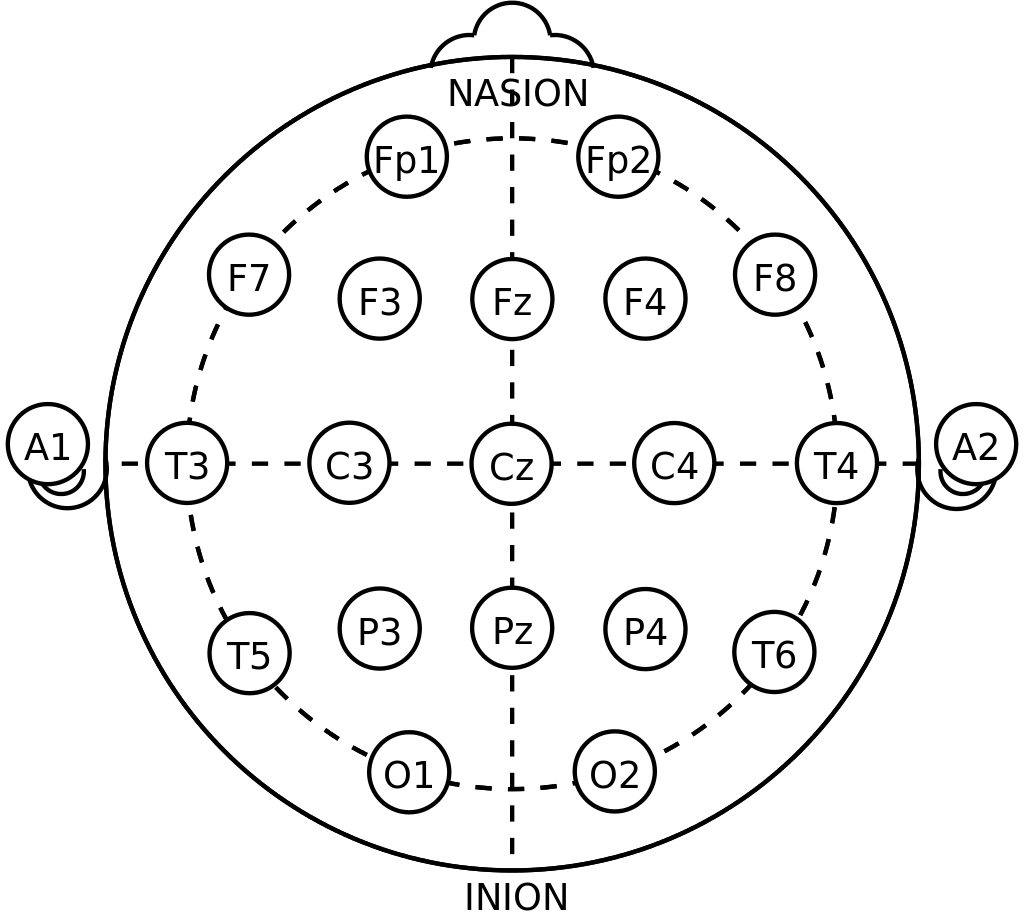
\includegraphics[width=1\linewidth]{src/20-10.png}
\caption{Стандартное расположение электродов на голове} %% подпись к рисунку
\label{pic:20-10} %% метка рисунка для ссылки на него
\end{minipage} \; \;
\begin{minipage}[h]{0.55\linewidth}
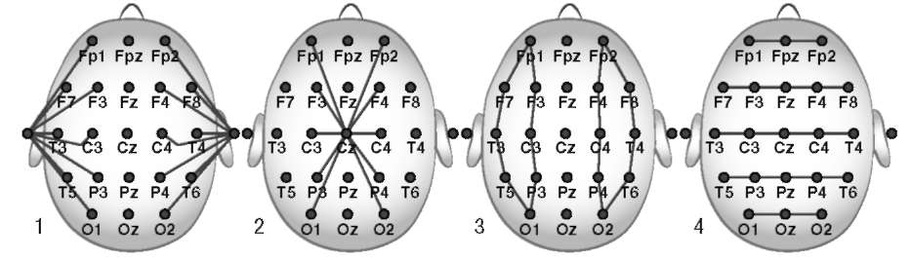
\includegraphics[width=1.2\linewidth]{src/Монтаж_ЭЭГ.jpg}
\caption{Различные способы соединять электроды между собой}
\label{pic:montage}
\end{minipage}
\end{center}
\end{figure}

Получаемый сигнал - это всегда разность напряжений между двумя электродами, поэтому каналы ЭЭГ обозначают, например, $Fp2 - A2$.
\end{frame}

\begin{frame}{Пример ЭЭГ сигнала}

\begin{figure}[h]
    \centering
    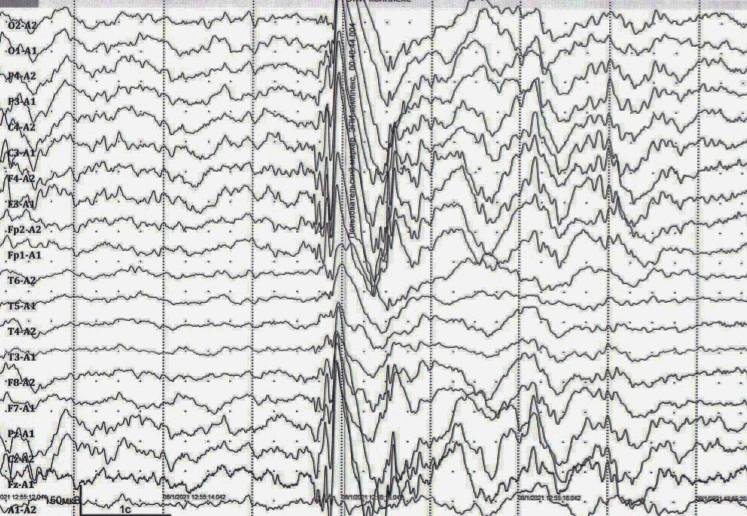
\includegraphics[width=1\linewidth]{src/ЭЭГ-с-эпилептической-активностью.jpg}
    \caption{Пример ЭЭГ с эпилептической активностью}
    \label{pic:epilepsy}
\end{figure}
    
\end{frame}

\begin{frame}{Ритмы ЭЭГ}

\begin{figure}[h]
    \centering
    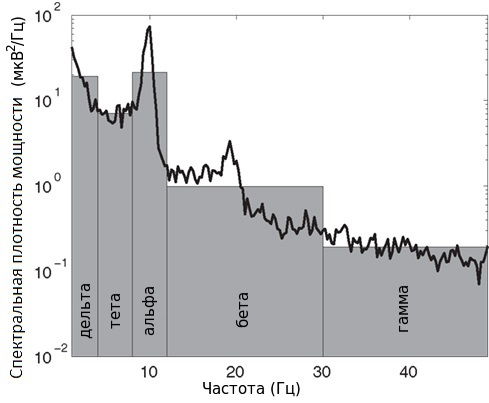
\includegraphics[width=0.75\linewidth]{src/Спектр_ЭЭГ.jpg}
    \caption{Разбиение спектра ЭЭГ на ритмы}
    \label{pic:rhythms}
\end{figure}
    
\end{frame}

\begin{frame}{Описание ритмов}

\begin{figure}
    \centering
    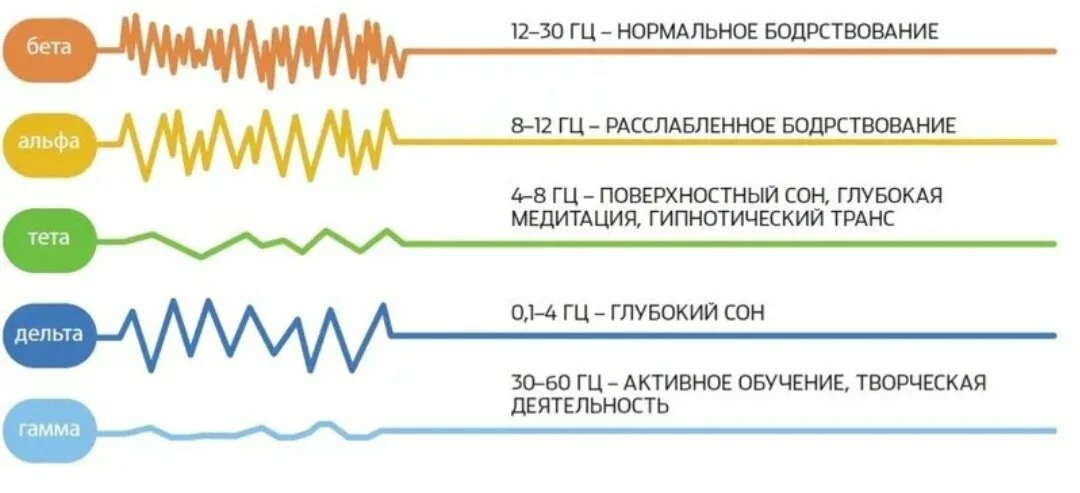
\includegraphics[width=1\linewidth]{src/Описание-ритмов.png}
    \caption{Описание часто встречаемых ритмов}
    \label{pic:rhythmes-depic}
\end{figure}
    
\end{frame}

\begin{frame}{Задание}

\begin{figure}
    \centering
    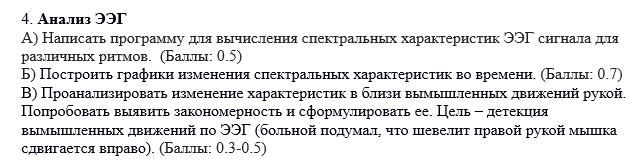
\includegraphics[width=1\linewidth]{src/Задание.png}
    \caption{Описание задания}
    \label{pic:task}
\end{figure}
    
\end{frame}

\begin{frame}{Ход работы}

1. Получение спектра на каждом промежутке времени
\begin{itemize}
    \item Для начала, условимся, что заданы $fs$ - частота дискретизации, $min_{hz}$ и $max_{hz}$ - диапазон частот, для которого мы будем проводить анализ (например, границы какого-нибудь ритма).
    \item Далее, мы разбиваем весь промежуток времени на $k$ неперескающихся отрезков, но считать все спектральные характеристики будем на $2k - 1$ пересекающихся наполовину отрезках, которые мы далее будем называть эпохами.
    \item Считаем спектр на каждом временном интервале и берем из него только частоты из диапазона.
\end{itemize}
    
\end{frame}

\begin{frame}{Ход работы}

2. Вычисление спектральных характеристик
\begin{itemize}
    \item Вычислим наибольшую амплитуду, частоту, на которой она достигается и среднюю амплитуду
    \item Затем вычислим средневзвешенную частоту $\overline{f}$
    $$
        \overline{f} = \frac{\sum\limits_{i = 1}^{n} f_i a_i}{\sum\limits_{i = 1}^{n} a_i},
    $$
    где $\{a_1, a_2, \ldots, a_n\}$ - это амплитуды, которые соответствуют частотам $\{f_1, f_2, \ldots, f_n\}$
\end{itemize}
    
\end{frame}

\begin{frame}{Ход работы}

3. Вычисление дополнительных характеристик сигнала
\begin{itemize}
    \item Вычислим энтропию сигнала на кусочке времени (на сколько сильно он колеблется, величина измеряется в битах)
    $$
        H(x) = - \sum\limits_{i=1}^{m} p_i \log_2 p_i,
    $$
    где $\{v_1, v_2, \ldots, v_m\}$ - множество значений, которые принимают амплитуды $a_j$, тогда $p_i$ - это эмпирическая вероятность того, что $a_j = v_i$, т.е. $p_i = \dfrac{\text{#} \{j \ | \ a_j = v_i\}}{n}$
\end{itemize}
    
\end{frame}

\begin{frame}{Ход работы}

4. Выделение особых проявлений ритмов и главного ритма в эпохе
\begin{itemize}
    \item Посчитаем <<силу>> ритма как интеграл (назовем это значение <<мощностью>> ритма в этой эпохе) при помощи формулы трапеций и будем считать, что у данного ритма в текущей эпохе происходит <<выброс>>, если его мощность в этой эпохе $>= \alpha * avr$, где $avr$ - средняя мощность по всем эпохам для этого ритма, а $\alpha$ - заранее выбранный коэффициент.
    \item Кроме того, найдем самый сильный ритм в этой эпохе, для этого просто выберем тот ритм, мощность которого наибольшая (уточнение - это не совсем справедливо, потому что средняя амплитуда на разных частотах очень сильно отличается - дельта-ритмы в 10-20 раз сильнее, например, гамма-ритмов).
\end{itemize}

\end{frame}

\begin{frame}{Ход работы}

5. Сравнение всех характеристик для двух электродов
\begin{itemize}
    \item Во-первых, можем продемонстрировать разность между двумя спектрограммами, чтобы найти, когда наблюдалась разность в частотах.
    \item Во-вторых сравним все предыдущие характеристики, можем искать отличия в подозрительных областях на тех частотах, которые покажутся нужными.
    \item Еще можем искать <<выбросы>> определенного ритма, которые есть только в первом сигнале, и их нет во втором и наоборот.
\end{itemize}
    
\end{frame}

\begin{frame}{Примеры из библиотеки MNE}

Библиотека MNE содержит большой набор размеченных данных (известны моменты времени, в которые, например, подавался звуковой сигнал в левое ухо) в формате .fif, в которых содержатся данные ЭЭГ и МРТ. Кроме этого, есть много механизмов для визуализации данных, обработки данных при помощи ML, спектрального анализа.

\hspace{20}

Далее приведем пример программы, которая считывает сырые данные, избавляется от артефактов записи используя ML, затем разбивает данные на эпохи (умнее, чем мы делали до этого). Затем можем отдельно посмотреть на некоторые каналы ЭЭГ и МРТ в те эпохи, когда был дан аудио сигнал - визуализировать сигнал и нарисовать спектр.

\end{frame}

\begin{frame}{Примеры из библиотеки MNE}

\begin{figure}[h]
    \centering
    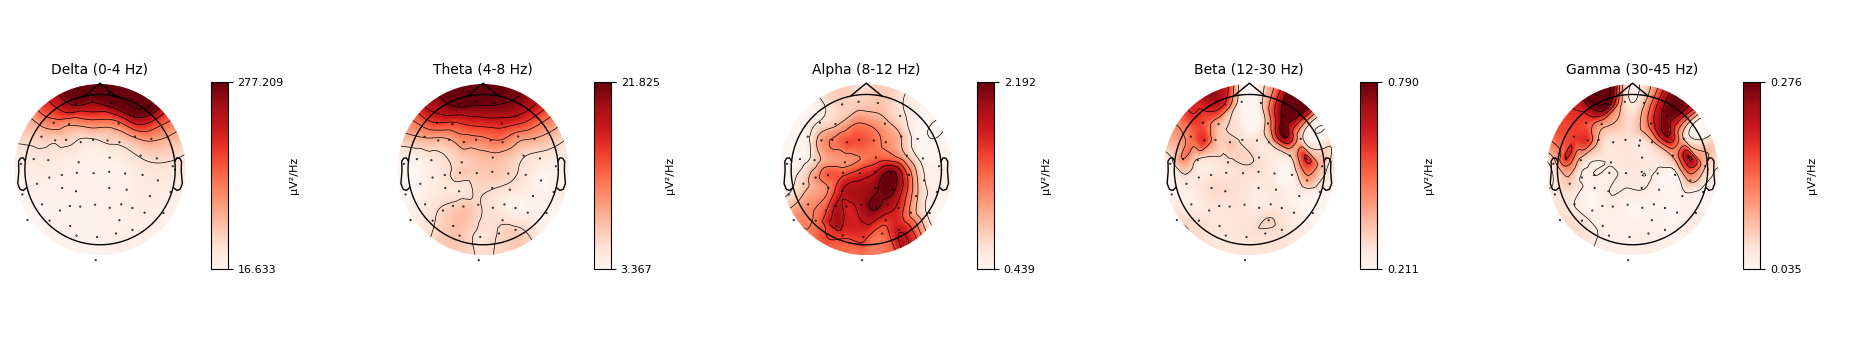
\includegraphics[width=1\linewidth]{src/Все-ритмы-MNE.png}
    \caption{Библиотека позволяет визуализировать в каких частях мозга были наиболее выражены определенные ритмы}
    \label{pic:mne}
\end{figure}

\begin{figure}[h]
    \centering
    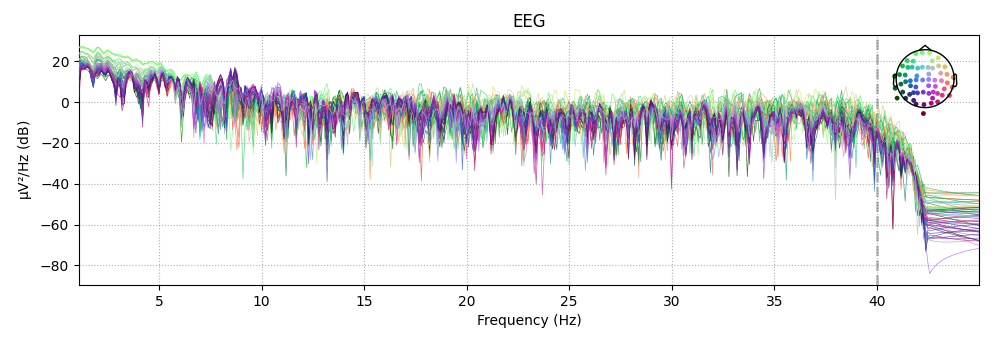
\includegraphics[width=1\linewidth]{src/Спектр-MNE.png}
    \caption{Красиво можем нарисовать спектр сразу нескольких каналов ЭЭГ}
    \label{pic:mne-spectrum}
\end{figure}
    
\end{frame}

\begin{frame}

\centering
{\huge
Спасибо за внимание!}

\hspace{30}

Найти исходники кода можно в репозитории:
\textcolor{blue}{\url{https://github.com/smellofnapalm/eeg-analysis}}
    
\end{frame}

\end{document}